\section{核形状指哪一种对象}\label{sec:1-2}

在经典几何中，物体的“形状”通常由表面边界、主轴长度与空间包络直观界定。然而，将这一概念平移至原子核体系时，立刻面临量子力学基本对称性的约束。原子核是由有限数目核子（质子与中子）依靠自洽强相互作用紧密束缚的孤立量子多体系统，典型线度在飞米量级。核力与电磁相互作用在孤立空间中满足空间旋转不变性，这使得核体系的哈密顿量与总角动量算符彼此对易。在通常的物理表象选择中，能量本征态可以同时选取为总角动量算符 $\hat{\mathbf{J}}^2$ 与其空间某一投影分量（例如 $\hat{J}_z$）的共同本征态。

这一机制引出一个核心疑问：偶偶核基态通常为自旋与宇称 $I^\pi = 0^+$，在实验室参考系中具有各向同性的空间取向。若单体电荷密度呈现球对称，核物理文献中广泛使用的长椭球、扁椭球或三轴椭球等几何形状概念，究竟对应哪一种真实的微观物理对象？

理解核形状概念需回到量子力学基本原理。首先从角动量三角条件出发，说明 $I=0$ 态的一阶实验室电四极矩为何必然消失，以及为何该零矩并不排除核子体系内部存在显著的空间四极关联；进而区分实验室密度、物质分布与内禀参考系，澄清将原子核类比为经典旋转刚体的认知局限；通过电四极旋转不变量方法，建立从实验室跃迁到形状参数的测量链条，并讨论量子涨落与实验截断对固定几何描述的实际限制。

\subsection{实验室系中的零矩与量子四极关联}\label{sec:1-2-1}

考察偶偶核最普遍的自旋 $I = 0$ 基态。在长波长极限与点核子一体近似下，描述点质子电荷空间分布的标准裸电四极张量算符 $\mathcal{M}(E2, \mu)$ 为二阶球张量（$L = 2$）：

\begin{equation}\label{eq:1-2-1}
\mathcal{M}(E2, \mu) = \int \hat{\rho}_c(\mathbf{r}) \, r^2 Y_{2\mu}(\theta, \phi) \, \mathrm{d}^3r = \sum_{k=1}^Z e \, r_k^2 Y_{2\mu}(\theta_k, \phi_k),
\end{equation}

其中 $\mathbf{r}_k$ 为各质子相对于核质心的位置，$e$ 为基本电荷，求和遍及 $Z$ 个质子。在截断模型空间中，核芯极化等被消去的自由度可通过有效算符近似计入。常用的一体有效电荷近似写为：

\begin{equation}\label{eq:1-2-2}
\hat{T}(E2, \mu) = \sum_{k\in\mathrm{active}} e_k^{\text{eff}} \, r_k^2 Y_{2\mu}(\theta_k, \phi_k),
\end{equation}

其中求和范围为模型中保留的活跃核子，质子和中子的有效电荷分别为 $e_p^{\text{eff}}$ 与 $e_n^{\text{eff}}$。这是一种有效算符近似，不能与完整空间的裸点质子算符不加区别地替换。

在实验室坐标系中，处于态 $|I, M\rangle$ 的能级其实验室静电四极矩（spectroscopic quadrupole moment）$Q_s(I)$ 定义为四极张量算符零分量在最大磁量子数 $M = I$ 上的期望值（包含传统几何因子 $\sqrt{16\pi/5}$）：

\begin{equation}\label{eq:1-2-3}
Q_s(I) \equiv \sqrt{\frac{16\pi}{5}} \, \langle I, M=I | \mathcal{M}(E2, 0) | I, M=I \rangle.
\end{equation}

由 Wigner--Eckart 定理 \cite{book-suhonen-from-nucleons-to-nucleus}，球张量算符的对角与非对角矩阵元可以分解为几何角动量耦合系数与约化矩阵元：

\begin{equation}\label{eq:1-2-4}
\langle I, M | \mathcal{M}(E2, \mu) | I, M' \rangle = (-1)^{I - M} \begin{pmatrix} I & 2 & I \\ -M & \mu & M' \end{pmatrix} \langle I || \mathcal{M}(E2) || I \rangle,
\end{equation}

其中矩阵括号内为 Wigner $3j$ 符号。该符号非零的一个必要条件是满足角动量三角定则 $\Delta(I, 2, I)$，即要求

\begin{equation}\label{eq:1-2-5}
|I - I| \le 2 \le I + I \implies 2I \ge 2 \implies I \ge 1.
\end{equation}

三角条件直接表明：对于任意 $I < 1$ 的量子态（特别是所有偶偶核的 $I=0$ 基态及 $I=1/2$ 能级），Wigner $3j$ 符号严格为零，其实验室静电四极矩必然恒为零：

\begin{equation}\label{eq:1-2-6}
Q_s(I=0) \equiv 0, \quad Q_s(I=1/2) \equiv 0.
\end{equation}

需要指出，$I \ge 1$ 只是解除了三角定则对非零静电四极矩的几何禁止，至于实际矩阵元是否显著偏离零，仍取决于约化矩阵元自身的微观大小。

对于具有确定空间宇称和角动量的孤立 $I=0$ 基态，若对其一体电荷密度算符求期望值，所得的空间分布必然是各向同性的：

\begin{equation}\label{eq:1-2-7}
\rho_{c, \text{lab}}(\mathbf{r}) \equiv \langle 0^+ | \hat{\rho}_c(\mathbf{r}) | 0^+ \rangle = \rho_0(r).
\end{equation}

然而，实验室一阶矩的消失并不表明核子在体系内部呈现刚性球形排布。一体电荷密度只是多粒子波函数在空间单点处的边缘几率分布，无法直接反映不同核子之间的相对空间角关联。

为了提取这种内部四极关联，可以考察电四极张量自身的标量缩并积（二阶不变量）：

\begin{equation}\label{eq:1-2-8}
\hat{A} \equiv \mathcal{M}(E2) \cdot \mathcal{M}(E2) = \sqrt{5} [\mathcal{M}(E2) \times \mathcal{M}(E2)]^0 = \sum_\mu (-1)^\mu \mathcal{M}(E2, \mu) \mathcal{M}(E2, -\mu).
\end{equation}

该算符在空间旋转下是标量算符，不受三角定则对角动量的相消限制。在 $I=0$ 态上插入能量本征态的完备中间基，该标量期望值 $q_2 = \langle \hat{A} \rangle$ 可以展开为跃迁强度的非负和：

\begin{equation}\label{eq:1-2-9}
q_2 = \langle 0^+ | \hat{A} | 0^+ \rangle = \sum_n |\langle 2_n^+ || \mathcal{M}(E2) || 0^+ \rangle|^2 = \sum_n B(E2; 0^+ \to 2_n^+) \ge 0.
\end{equation}

这一关系表明，只要基态与低激发四极态之间存在显著的相干 $E2$ 跃迁强度，二阶标量期望值就会显著大于零。因此，实验室系中观察到的球对称性反映的是孤立体系整体取向的各向同性，而核体系内部完全可以容纳强烈的相对四极空间关联。

\subsection{密度的描述层次：实验室态、物质分布与内禀坐标}\label{sec:1-2-2}

在研究核形状时，需区分不同物理层次的描述对象。首先是一体密度与多粒子关联的差异。电子弹性散射测量的一体电荷密度 $\rho_c(\mathbf{r})$ 是对其余粒子坐标积分后的边缘几率分布，反映电荷半径与径向弥散，但无法直接提供相对方位的角关联。相比之下，核子间的空间相关性体现在二体及高阶密度矩阵中，例如二粒子关联函数：

\begin{equation}\label{eq:1-2-10}
\rho^{(2)}(\mathbf{r}_1, \mathbf{r}_2) = \langle \Psi | \sum_{i \ne j} \delta(\mathbf{r}_1 - \mathbf{r}_i) \delta(\mathbf{r}_2 - \mathbf{r}_j) | \Psi \rangle.
\end{equation}

即便单体密度 $\rho_c(\mathbf{r})$ 各向同性，两粒子相对夹角 $\theta_{12}$ 的分布仍可偏离无角关联的参考分布，并保留四极关联。这里应比较相同角测度下的分布；各向同性并不意味着关于 $\theta_{12}$ 本身的概率密度为常数。二次四极标量也含同一核子的自项，单凭其非零还不能判断集体相干性的强弱。

其次需要明确电荷分布与物质分布的区别。通常的在束 $\gamma$ 跃迁与库仑激发实验直接探测由带电质子贡献的电荷四极性质；而决定自洽平均场势阱的则是全体核子参与的强相互作用物质分布：

\begin{equation}\label{eq:1-2-11}
\hat{\rho}_m(\mathbf{r}) = \sum_{k=1}^A \delta(\mathbf{r} - \mathbf{r}_k) = \hat{\rho}_p(\mathbf{r}) + \hat{\rho}_n(\mathbf{r}).
\end{equation}

在宏观均质流体假设下，人们有时假定电荷四极算符正比于物质四极算符：$\mathcal{M}(E2) \approx \frac{eZ}{A} \hat{Q}_2^{(m)}$。但在微观核体系中，该比例关系并不普遍成立。质子与中子分别占据不同单粒子壳层，其费米面与形变驱动效应往往并不对称；在远离稳定线的中子过剩核中，价中子可强烈驱动四极或三轴形变，而质子核芯具有不同的极化刚度。此外，电磁跃迁中还包含核子反常磁矩贡献（如 $M1$ 跃迁），并非所有辐射寿命均由质子电荷流决定。微观计算中通常需引入有效电荷与极化因子以补偿空间截断效应。因此，讨论核形状时须严格指明所考察的是由电磁跃迁界定的电荷形状，还是由全体核子空间分布界定的物质形状。

最后需要澄清有效内禀参考系的物理地位。为了描述核多体波函数中的相干四极关联，Aage Bohr \cite{bohr-1952-surface-particle-coupling} 引入了瞬时主轴参考系。该方法利用 Wigner $D$ 矩阵旋转变换，将实验室系的 5 个实空间四极形变变量 $\alpha_\mu$（$\mu=-2..2$）变换为主轴参考系的 3 个取向欧拉角 $\theta_i$ 以及 2 个描写内部形状的参数：

\begin{equation}\label{eq:1-2-12}
a_0 = \beta \cos\gamma, \quad a_2 = a_{-2} = \frac{1}{\sqrt{2}} \beta \sin\gamma, \quad a_1 = a_{-1} = 0.
\end{equation}

这里，$\beta$ 表征总偏离球形的形变幅度，而 $\gamma$ 表征偏离轴对称性的三轴度参数。

在理解这一几何框架时，需警惕机械的经典图景：将原子核视为形状固定、在空间中高速旋转的经典刚体，而将实验室观测到的球对称性归结为“长时间曝光留下的模糊圆影”。经典曝光类比可作为理解空间平均的认知脚手架，但不能取代真实的微观量子图景。在孤立微观体系中，内禀坐标并非惯性参考系，而是描述集体运动的辅助坐标；它不仅用于构建破缺平均场参考态，也广泛用于显式量子集体哈密顿量、角动量投影态与条件概率分布分析；核波函数在内部坐标 $(\beta, \gamma)$ 上展现为具有有限弥散度的分布，而非单一的几何极值点；同时，原子核转动涉及多核子的微观组态调整与配对关联，不同于经典刚体运动。

\subsection{实验测度：Kumar--Cline 旋转不变量理论}\label{sec:1-2-3}

为了建立摆脱特定唯象模型假设的客观测量链条，Douglas Cline 与 Krishna Kumar 发展了电四极旋转不变量方法 \cite{cline-1986-nuclear-shapes-coulomb-excitation}。

该方法的基本逻辑是：通过角动量耦合，将实验室系测量的电四极张量算符 $\mathcal{M}(E2)$ 缩并为空间旋转标量算符。这些标量算符在实验室系中的期望值，在数学上等同于它们在瞬时主轴系中的空间分布期望值。

在瞬时主轴参考系中，电四极张量仅有两个独立的非零主轴参数。Cline 在其评述中 \cite{cline-1986-nuclear-shapes-coulomb-excitation} 采用四极幅度 $Q$ 与不对称角参数 $\delta$ 进行描写。为了与后文描述电磁跃迁中多极发射振幅比（光子混合比）的常用符号 $\delta$ 明确区分，本节及后续章节将该形状角统一定义并映射为标准三轴角 $\gamma$（即令 $\delta \equiv \gamma$）：

\begin{equation}\label{eq:1-2-13}
E(2, 0) = Q \cos\gamma, \quad E(2, 2) = E(2, -2) = \frac{1}{\sqrt{2}} Q \sin\gamma, \quad E(2, 1) = E(2, -1) = 0.
\end{equation}

依据所采用的可交换电四极坐标与张量标量积归一，最低阶的两个核心不变量定义为：

\begin{equation}\label{eq:1-2-14}
q_2 \equiv \sqrt{5} \, \langle s | [\mathcal{M}(E2) \times \mathcal{M}(E2)]^0 | s \rangle = \langle s | \hat{A} | s \rangle = \langle s | Q^2 | s \rangle,
\end{equation}

\begin{equation}\label{eq:1-2-15}
q_3 \equiv -\sqrt{\frac{35}{2}} \, \langle s | [[\mathcal{M}(E2) \times \mathcal{M}(E2)]^2 \times \mathcal{M}(E2)]^0 | s \rangle = \langle s | \hat{B} | s \rangle = \langle s | Q^3 \cos(3\gamma) | s \rangle.
\end{equation}

对于具有实际物理量纲的跃迁算符，\textbf{$q_2$ 的单位为 $e^2\,\mathrm{fm}^4$}，反映总四极形变平方的大小；\textbf{$q_3$ 的单位为 $e^3\,\mathrm{fm}^6$}，反映三轴不对称度与形变立方的相干乘积。这里需要说明记号约定：$q_3$ 本身已是电四极张量的三次相干不变量，定义中包含三倍角余弦项 $\cos(3\gamma)$，不应写作 $q_3^3$ 或改变代数符号。在标准第一不可约扇区（$0^\circ \le \gamma \le 60^\circ$）内，对于轴对称长椭球（$\gamma = 0^\circ$），$q_3 > 0$；对于轴对称扁椭球（$\gamma = 60^\circ$），$q_3 < 0$；而对于 $\gamma = 30^\circ$ 的中点对称几何，三次不变量 $q_3$ 严格消失。

旋转不变量的核心价值在于：通过插入完备中间态，这些标量期望值可精确展开为可测约化矩阵元网络的求和。例如，$q_2$ 由态 $|s\rangle$ 通往各中间态的约化矩阵元平方和直接给出；而三次不变量 $q_3$ 则包含不同激发态间的相互跃迁及激发态静态电四极矩（重取向效应），并显著依赖于矩阵元间的相对代数相位 \cite{cline-1986-nuclear-shapes-coulomb-excitation}。重离子多步库仑激发实验正是通过测量能级布居截面，系统提取包含对角与非对角跃迁的矩阵元网络。

需要强调实验适用边界：多步库仑激发约束的是低能有限自由度的离散 $E2$ 矩阵元网络，并不直接等同于连续三维电荷密度的空间重构。在实际求和中，数据必须在有限低能级截断；该截断之所以能较好反映低频集体四极特征，依赖于低频集体模与高能巨四极共振（GQR）动力学上的弱耦合分离。

\IfFileExists{Img/shape-moments.pdf}{
\begin{figure}[htbp]
\centering
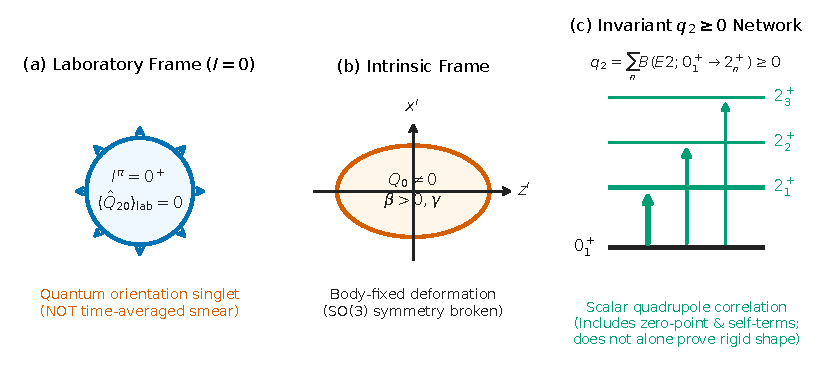
\includegraphics[width=.92\textwidth]{Img/shape-moments.pdf}
\caption{微观核电荷四极形状、主轴参考系与二阶、三阶旋转不变量概念示意图。}\label{fig:shape-moments}
\end{figure}
}{}

\subsection{矩比、量子涨落与几何描述的适用边界}\label{sec:1-2-4}

在求得二次矩 $q_2$ 与三次矩 $q_3$ 后，常采用二者之比定义有效形状角：

\begin{equation}\label{eq:1-2-16}
\cos(3\gamma_{\text{eff}}) \equiv \frac{q_3}{q_2^{3/2}} = \frac{\langle \hat{B} \rangle}{\langle \hat{A} \rangle^{3/2}}.
\end{equation}

需要明确指出：仅当 $q_2 > 0$ 且比值落在实数区间 $\left| q_3 / q_2^{3/2} \right| \le 1$ 时，上式才允许通过反余弦函数反解出实数的有效角 $\gamma_{\text{eff}}$。比值 $q_3 / q_2^{3/2}$ 并非角度函数 $\cos(3\gamma)$ 的无权几何平均，因为其分母为 $\langle \hat{A} \rangle^{3/2}$ 而非 $\langle Q^3 \rangle$。在一般的径向涨落下，由于幅度与角度的相干关联，该比值完全可能超出 $[-1, 1]$。例如在一个正权可交换坐标的教学控制模型中（非实核数据），设体系在角度上固定为轴对称长椭球 $\gamma = 0^\circ$（即 $\cos 3\gamma \equiv 1$），而在幅度上存在两点等几率涨落：$Q = 1$ 与 $Q = 2$ 各占 $1/2$ 几率；此时可算得 $\langle \hat{A} \rangle = \frac{1^2 + 2^2}{2} = 2.5$，$\langle \hat{B} \rangle = \frac{1^3 + 2^3}{2} = 4.5$，矩比为 $\frac{4.5}{(2.5)^{3/2}} = \frac{9\sqrt{10}}{25} \approx 1.138 > 1$，反余弦在实数域无解。这表明不能将该矩比简单视为角度的有界平均，在缺乏波包分布先验信息时，仅凭该矩比不能直接断定体系处于刚性极小势阱还是软势面摆动。

给微观量子态赋予单一固定几何形状具有明确适用条件。利用四阶标量算符 $\hat{A}^2 = (\mathcal{M}(E2) \cdot \mathcal{M}(E2))^2$ 定义的形变相对宽度

\begin{equation}\label{eq:1-2-17}
\frac{\Delta A}{\langle \hat{A} \rangle} \equiv \frac{\sqrt{\langle \hat{A}^2 \rangle - \langle \hat{A} \rangle^2}}{\langle \hat{A} \rangle}
\end{equation}

直接量化了态上径向四极幅度的微观量子涨落 \cite{poves-2020-limits-assigning-nuclear-shape}。需要强调，这一相对宽度衡量的是径向幅度的量子涨落，并不反映三轴角 $\gamma$ 的定域程度，更不是实验测量的统计估计误差；在一般算符实现中不能未声明就将它写为 $Q$，仅在经典/可交换坐标实现下才对应于 $\hat{A} = Q^2$。

Poves 等人用指定CI模型的质量四极算符考察了这一问题，其结果不是实测电荷涨落：Table I中 $^{24}\mathrm{Mg}$ 基态的相对宽度为0.25，$^{34}\mathrm{Si}$ 基态为1.07。它们说明在所考察的态与算符下，固定几何描述可以具有很不相同的精度。宽幅度分布使单一构型难以概括波函数，但它本身也不证明存在某种确定的动态振动。反之，规则转动谱或窄的径向涨落均不能单独推出深势阱、局域的 $\gamma$ 或固定惯量。较大的 $q_2$ 和超过 Weisskopf 单粒子估计的 $B(E2)$ 也可出现在振动、组态混合或软核模型中，须结合其它观测解释。

表~\ref{tab:1-2-shape-hierarchy}辨析了本节讨论的三种不同描述层次及其特征：

\begin{table}[htbp]
\centering
\small
\caption{核形状在微观核物理中的描述层次、对称性与实验提取途径}\label{tab:1-2-shape-hierarchy}
\begin{tabularx}{\textwidth}{p{2.6cm}p{3.0cm}p{2.6cm}p{2.8cm}X}
\toprule
描述层次 & 物理载体 & 对称性特征 & 实验观测与提取途径 & 适用边界与物理局限 \\
\midrule
\textbf{实验室一体密度} $\rho_{c, \text{lab}}(\mathbf{r})$ & 单粒子电荷密度算符在实验室能量本征态上的期望值 & 各向同性（$I=0$ 态），空间球对称 & 电子弹性散射、缪子 X 射线光谱 & 反映单体边缘几率，不直接展现两体相干角关联 \\
\textbf{有效内禀形状参数} $(\beta, \gamma)$ & 瞬时主轴参考系下的集体模型或平均场坐标 & 参考构型可不具轴对称性，精确态保持转动对称 & 理论模型映射参量，无法在实验室系直接测量 & 在波包定域时支持固定几何赋值；在软核或振动核中主要作为有效动态幅度 \\
\textbf{旋转不变量矩阵网络} $(q_2, q_3, \dots)$ & 空间旋转不变的电四极张量算符零耦合标量缩并积 & 标量不变量，对实验室空间旋转不变 & 重离子多步库仑激发多体跃迁与对角矩求和 & 受限于低能激发态有限截断与实验误差；反映离散矩阵元网络而非连续空间断层扫描 \\
\bottomrule
\end{tabularx}
\end{table}

上述分析表明，“核形状”在量子力学框架下并非宏观刚性边界在微观的简单复制，而是多体波函数内部相干空间四极关联的宏观投影，在实验室观测中具体实现为一系列可测量的旋转标量算符期望值。

这一认识为后续各章的理论展开提供了切入点。关于实验室对称性、约化矩阵元代数以及上下行跃迁强度的统计权关系，将在第~\ref{sec:2-1}~节中结合 Wigner--Eckart 定理与张量语言系统推导；内部形状坐标 $(\beta, \gamma)$、度规张量与动能微分算符的严格微分几何测度，将在第~\ref{sec:2-4}~节中展开；静态几何形变与集体转动惯量的微观响应差异，将在第~\ref{sec:2-6}~节中通过自洽场与配对结构深入探讨；而多步库仑激发矩阵元网络的反演技术、探测器响应与截断不确定度评估，则将在第~5~章中结合完整实验技术链详细阐述。
